\documentclass[tikz,border=10pt]{standalone}
\usetikzlibrary{shapes}
\usetikzlibrary{arrows}
\usetikzlibrary{positioning}
\begin{document} 

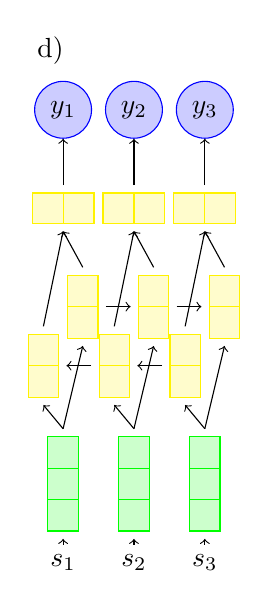
\begin{tikzpicture}[
  hid/.style 2 args={
    rectangle split,
    draw=#2,
    rectangle split parts=#1,
    fill=#2!20,
    outer sep=1mm},
  mlp/.style 2 args={
    rectangle split,
    rectangle split horizontal,
    draw=#2,
    rectangle split parts=#1,
    fill=#2!20,
    outer sep=1mm}
]

  \node [anchor=west] (label) at (.45, 4.5) {d)};
 \foreach \i [count=\step from 1] in {$s_1$, $s_2$, $s_3$}
    \node (i\step) at (.9*\step, -2) {\i};
  % draw embedding and hidden layers for text input
  \foreach \step in {1,...,3} {
    \node[hid={3}{green}] (e\step) at (.9*\step, -1) {};    
    \draw[->] (i\step.north) -> (e\step.south);
  }

  \foreach \step in {1,...,3} {
    \node[hid={2}{yellow}] (h_r_\step) at (-.25 + .9 *\step, .5) {};    
    \node[hid={2}{yellow}] (h_f_\step) at (.25 + .9 *\step, 1.25) {};    
    \draw[->] (e\step.north) -> (h_f_\step.south);
    \draw[->] (e\step.north) -> (h_r_\step.south);
    \node[mlp={2}{yellow}] (h_\step) at (.9 *\step, 2.5) {};    
    \node[circle, draw=blue, fill=blue!20] (y_\step) at (.9 *\step, 3.75) {$y_\step$};    
    \draw[->] (h_\step.north) -> (y_\step.south);
    \draw[->] (h_f_\step.north) -> (h_\step.south);
    \draw[->] (h_r_\step.north) -> (h_\step.south);
  }

  \foreach \step/\steppp in {1/2, 2/3} {
    \draw[->] (h_f_\step.east) -> (h_f_\steppp.west);
    \draw[->] (h_r_\steppp.west) -> (h_r_\step.east);
  }
 

\end{tikzpicture}


\end{document}
